Now having three successful models that are able to predict GFP fluorescence from the whole cell, nuclei and ER, one can combine their predictions for the same image. To do that an output RGB image was constructed, where each prediction takes one channel. The resulting image is shown in Figure \ref{fig:combined}. Additionally one can see that the GFP model has successfully generalized on other cell phenotypes (CHOZN, PHX). Originally this model was trained on H19 phenotype only, however predictions for two other phenotypes (see Figure  \ref{fig:combined} PHX, CHOZN) highlight the cell area successfully as well.

\begin{figure}[htb]
	\begin{center}
		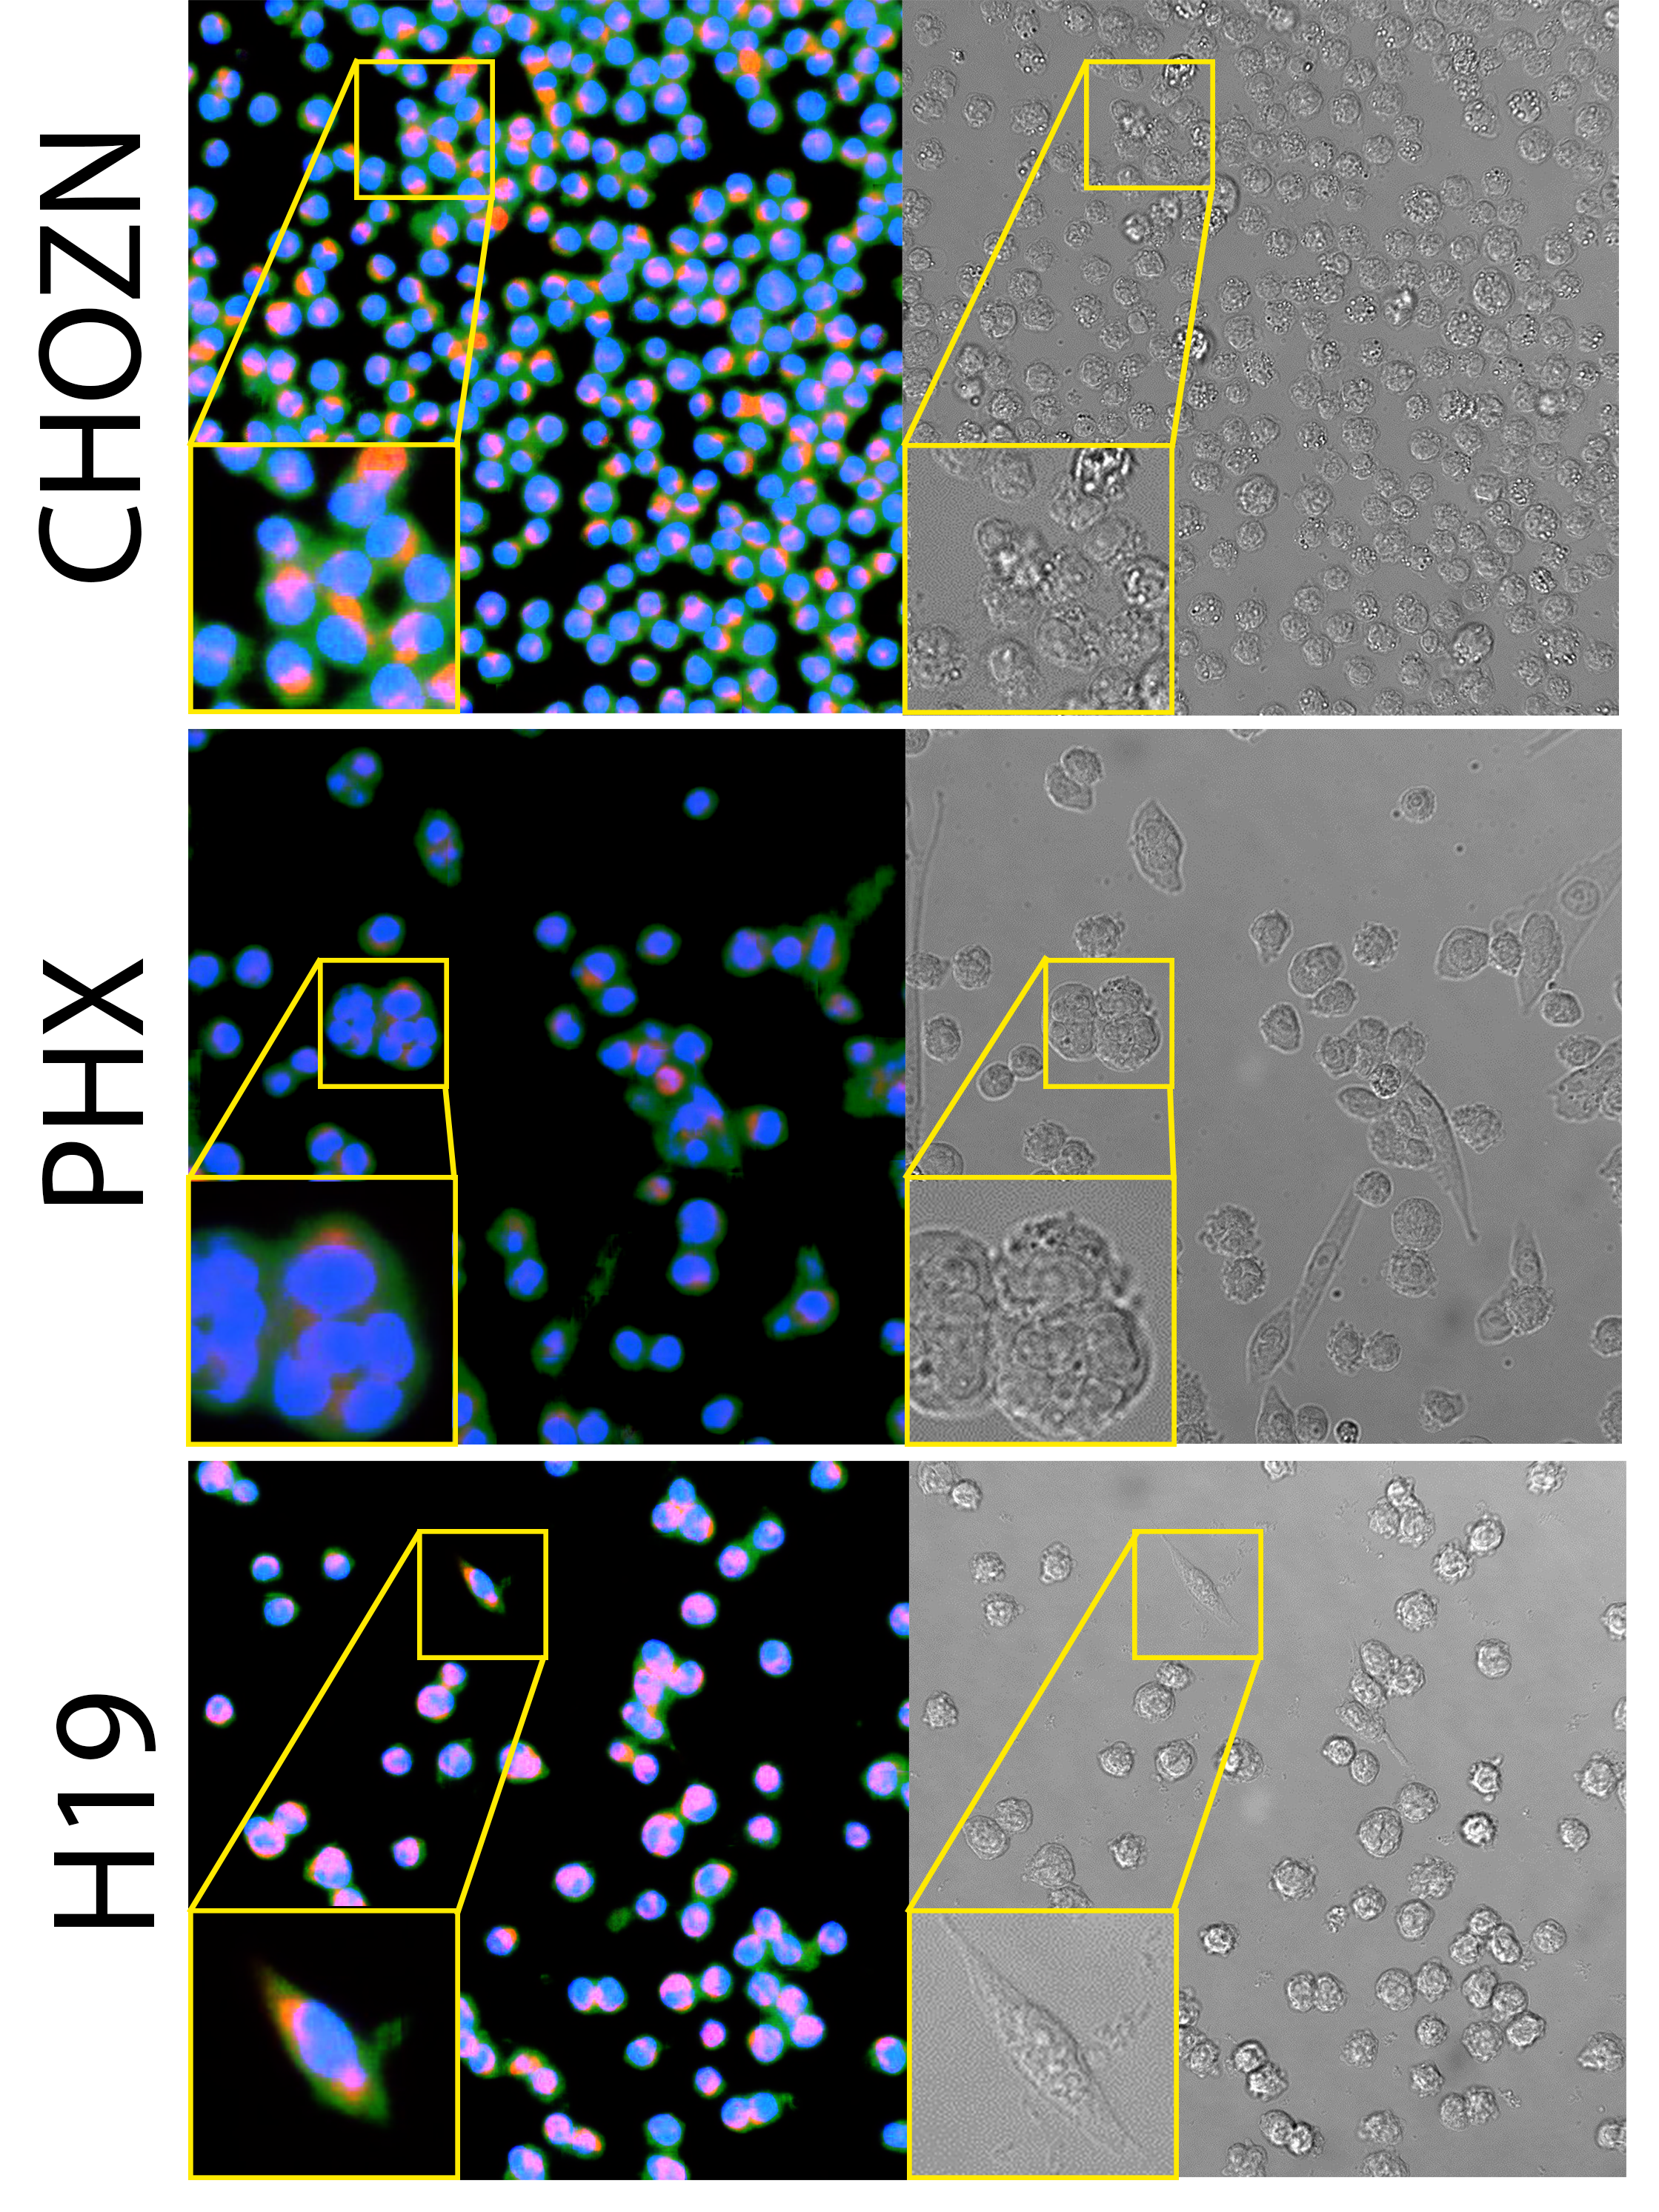
\includegraphics[width=0.85\linewidth]{bilder/combined/combined.png}
		\caption[GFP, Nuclei and ER combined]%
		{Combination of predictions of three UNets: GFP, nuclei and ER. Each organelle occupies one RGB channel: red --- ER, green --- GFP, blue --- nuclei.}\label{fig:combined}
	\end{center}
\end{figure}
